\documentclass[11pt]{article}
\usepackage{graphicx}
\usepackage{times}
\pagestyle{myheadings}
\addtolength{\topmargin}{-0.75in}
\author{Emden R. Gansner and Eleftherios Koutsofios and Stephen North}
\def\dot{{\it dot}}
\def\dag{{\it dag}}
\def\DOT{{\it DOT}}
\def\graphviz{{\it Graphviz}}
\newcommand{\lastedited}{January 5, 2015}
\date{\lastedited}
\newcommand{\mymark}{{\it dot} User's Manual, \lastedited \hfil }
\markboth{\mymark}{\mymark}
\begin{document}
\bibliographystyle{alpha}
\title{Drawing graphs with \dot}
\maketitle
\begin{abstract}
\noindent
{\dot} draws directed graphs as hierarchies.
It runs as a command line program, web visualization
service, or with a compatible graphical interface.
Its features include well-tuned layout algorithms
for placing nodes and edge splines, edge labels,
``record'' shapes with ``ports'' for drawing data structures;
cluster layouts; and an underlying file language for
stream-oriented graph tools.
Below is a reduced module dependency graph of an SML-NJ compiler
that took 0.23 seconds of user time on a 3 GHz Intel Xeon.

\vspace*{.25in}
\centerline{
	\includegraphics[width=4.0in]{smlred}
}
\end{abstract}

\newpage
\section{Basic Graph Drawing}
\dot\ draws directed graphs. It reads attributed graph text files and
writes drawings, either as graph files or in a graphics format
such as GIF, PNG, SVG, PDF, or PostScript.


\if 0
{\bf 
All details are here and up-to-date.
The question is which, if any, should be removed,
and should the document structure be changed. Some of the
appendices might belong in the main body, and parts of the main
body (e.g., the attribute tables and command line information) 
might be better in the appendix. Maybe the Node and Edge Placement
section should appear before Drawing Size and Spacing.
\fi

\dot\ draws graphs in four main phases.
Knowing this helps you to understand what kind of
layouts \dot\ makes and how you can control them.
The layout procedure used by \dot\ relies on the graph
being acyclic. Thus, the first step is to break any
cycles which occur in the input graph by reversing
the internal direction of certain cyclic edges.
The next step assigns nodes to discrete ranks or levels.
In a top-to-bottom drawing, ranks determine $Y$ coordinates.
Edges that span more than one rank are broken into chains
of ``virtual'' nodes and unit-length edges.
The third step orders nodes within ranks to avoid crossings.
The fourth step sets $X$ coordinates of nodes to keep edges short,
and the final step routes edge splines.
This is the same general approach as most hierarchical graph drawing
programs, based on the work of Warfield \cite{warfield},
Carpano \cite{carpano} and Sugiyama \cite{stt}.
We refer the reader to \cite{gknv:methods}
for a thorough explanation of \dot's algorithms.

\dot\ accepts input in the \DOT\ language (cf. Appendix~\ref{grammar}). 
This language describes three main kinds of objects:
graphs, nodes, and edges.
The main (outermost) graph can be directed
({\tt digraph}) or undirected {\tt graph}.
Because \dot\ makes layouts of directed graphs,
all the following examples use {\tt digraph}.
(A separate layout utility, {\it neato},
draws undirected graphs \cite{neatoguide}.)
Within a main graph, a {\tt subgraph} defines a
subset of nodes and edges.

Figure~\ref{fig:graph1} is an example graph in the \DOT\ language. 
Line 1 gives the graph name and type.
The lines that follow create nodes, edges, or subgraphs,
and set attributes. Names of all these objects may be
C identifiers, numbers, or quoted C strings.
Quotes protect punctuation and white space.

\begin{figure}[p]
\begin{verbatim}
1:  digraph G {
2:      main -> parse -> execute;
3:      main -> init;
4:      main -> cleanup;
5:      execute -> make_string;
6:      execute -> printf
7:      init -> make_string;
8:      main -> printf;
9:      execute -> compare;
10: }
\end{verbatim}
\caption{Small graph}
\label{fig:graph1}
\end{figure}

\begin{figure}[p]
	\centerline {
		\includegraphics[width=3.0in]{graph1}
	}
    \caption{Drawing of small graph}
    \label{fig:drawing1}
\end{figure}

A node is created when its name first appears in the file.
An edge is created when nodes are joined by the edge operator \verb"->".
In the example, line 2 makes edges from {\it main} to {\it parse},
and from {\it parse} to {\it execute}.
Running \dot\ on this file (call it \verb"graph1.gv")
\begin{verbatim}
    $ dot -Tps graph1.gv -o graph1.ps
\end{verbatim}
yields the drawing of Figure~\ref{fig:drawing1}.
The command line option \verb"-Tps" selects PostScript (EPSF) output. 
\verb"graph1.ps" may be printed, displayed by a PostScript viewer,
or embedded in another document.

It is often useful to adjust the representation or placement of nodes
and edges in the layout.  This is done by setting attributes of nodes,
edges, or subgraphs in the input file.
Attributes are name-value pairs of character strings.
Figures~\ref{fig:graph2} and \ref{fig:drawing2} illustrate
some layout attributes.  In the listing of Figure~\ref{fig:graph2},
line 2 sets the graph's {\tt size} to {\tt 4,4}
(in inches).
This attribute controls the size of the drawing; if the drawing is
too large, it is scaled uniformly as necessary to fit.

Node or edge attributes are set off in square brackets.
In line 3, the node \verb"main" is assigned shape \verb"box".
The edge in line 4 is straightened by increasing its 
\verb"weight" (the default is \verb"1").
The edge in line 6 is drawn as a dotted line.
Line 8 makes edges from {\tt execute} to {\tt make\_string} and {\tt printf}.
In line 10 the default edge color is set to \verb"red".
This affects any edges created after this point in the file.
Line 11 makes a bold edge labeled {\tt 100 times}.
In line 12, node \verb"make_string" is given a multi-line label.
Line 13 changes the default node to be a box filled with a shade of blue.
The node {\tt compare} inherits these values.

\begin{figure}[p]
\begin{verbatim}
1:  digraph G {
2:      size ="4,4";
3:      main [shape=box];   /* this is a comment */
4:      main -> parse [weight=8];
5:      parse -> execute;
6:      main -> init [style=dotted];
7:      main -> cleanup;
8:      execute -> { make_string; printf}
9:      init -> make_string;
10:     edge [color=red];   // so is this
11:     main -> printf [style=bold,label="100 times"];
12:     make_string [label="make a\nstring"];
13:     node [shape=box,style=filled,color=".7 .3 1.0"];
14:     execute -> compare;
15: }
\end{verbatim}
\caption{Fancy graph}
\label{fig:graph2}
\end{figure}

\begin{figure}[p]
	\centerline {
		\includegraphics[width=2.5in]{graph2}
	}
    \caption{Drawing of fancy graph}
    \label{fig:drawing2}
\end{figure}

\section{Drawing Attributes}

The main attributes that affect graph drawing
are summarized in Appendices~\ref{sec:node_attr}, 
\ref{sec:edge_attr} and \ref{sec:graph_attr}.
For more attributes and a more complete description of the attributes, you
should refer to the \graphviz\ web site, specifically
\begin{center}
{\tt www.graphviz.org/doc/info/attrs.html}
\end{center}

\subsection{Node Shapes}
\label{sect:shape}

Nodes are drawn, by default, with {\tt shape=ellipse}, {\tt width=.75},
{\tt height=.5} and labeled by the node name.
Other common shapes include {\tt box}, {\tt circle}, {\tt record} 
and {\tt plaintext}.
A list of the main node shapes is given in Appendix~\ref{app:shapes}.
The node shape {\tt plaintext} is of particularly interest in
that it draws a node without any outline, an important convention
in some kinds of diagrams. In cases where the graph structure is of
main concern, and especially when the graph is moderately large, the
{\tt point} shape reduces nodes to display minimal content.
When drawn, a node's actual size is the greater of the requested
size and the area needed for its text label, unless {\tt fixedsize=true},
in which case the {\tt width} and {\tt height} values are enforced.

Node shapes fall into two broad categories: polygon-based and
record-based.\footnote{There is a way to implement custom node shapes,
using {\tt shape=epsf} and the {\tt shapefile} attribute, and
relying on PostScript output.
The details are beyond the scope of this user's guide.
Please contact the authors for further information.} All node
shapes except {\tt record} and {\tt Mrecord} are considered polygonal,
and are modeled by the number of sides (ellipses and circles being
special cases), and a few other geometric properties. Some of these
properties can be specified in a graph. If {\tt regular=true}, the
node is forced to be regular. The parameter {\tt peripheries} sets
the number of boundary curves drawn. For example, a doublecircle 
has {\tt peripheries=2}.
The {\tt orientation} attribute specifies a clockwise rotation of the 
polygon, measured in degrees.

The shape {\tt polygon} exposes all the polygonal parameters, and
is useful for creating many shapes that are not predefined.
In addition to the parameters {\tt regular}, {\tt peripheries} and
{\tt orientation}, mentioned above, polygons are parameterized by 
number of sides {\tt sides}, {\tt skew} and {\tt distortion}.
{\tt skew} is a floating point number (usually between $-1.0$ and $1.0$)
that distorts the shape by slanting it from top-to-bottom,
with positive values moving the top of the polygon to the right.
Thus, {\tt skew} can be used to turn a box into a parallelogram.
{\tt distortion} shrinks the polygon from top-to-bottom, with negative
values causing the bottom to be larger than the top. {\tt distortion}
turns a box into a trapezoid. A variety of these polygonal attributes
are illustrated in Figures~\ref{fig:polygons} and~\ref{fig:polylist}.

\begin{figure}[p]\footnotesize
\begin{verbatim}
1:  digraph G {
2:      a -> b -> c;
3:      b -> d;
4:      a [shape=polygon,sides=5,peripheries=3,color=lightblue,style=filled];
5:      c [shape=polygon,sides=4,skew=.4,label="hello world"]
6:      d [shape=invtriangle];
7:      e [shape=polygon,sides=4,distortion=.7];
8:  }
\end{verbatim}
\caption{Graph with polygonal shapes}
\label{fig:polylist}
\end{figure}
\begin{figure}[p]
	\centerline {
		\includegraphics{poly}
	}
    \caption{Drawing of polygonal node shapes}
    \label{fig:polygons}
    \vspace*{.5in} % tweak to make this figure use rest of page
\end{figure}

Record-based nodes form the other class of node shapes. 
These include the
shapes {\tt record} and {\tt Mrecord}. The two are identical
except that the latter has rounded corners. These nodes represent
recursive lists of fields, which are drawn as alternating horizontal
and vertical rows of boxes. The recursive structure is determined by
the node's {\tt label}, which has the following schema: \\
\begin{table}[h]
\begin{tabular}{lll}
{\it rlabel}  & $\rightarrow$ & {\it field} ( '$|$' {\it field} )* \\
{\it field}  & $\rightarrow$ & {\it boxLabel} $|$ '{' {\it rlabel} '}' \\
{\it boxLabel}  & $\rightarrow$ & [ '$<$' {\it string} '$>$' ] [ {\it string} ] \\
\end{tabular}
\end{table}

Literal braces, vertical bars and angle brackets must be escaped. 
Spaces are interpreted as separators between tokens, so they
must be escaped if they are to appear literally in the text.
The first string in a {\it boxLabel} gives a name to the field,
and serves as a port name for the box (cf. Section~\ref{sect:ports}).
The second string is used as a label for the field; 
it may contain the same escape sequences as multi-line 
labels (cf. Section~\ref{sect:labels}).
The example of Figures~\ref{fig:record} and \ref{fig:recorddrawing}
illustrates the use and some properties of records.

\begin{figure}[p]\footnotesize
\begin{verbatim}
1:  digraph structs {
2:  node [shape=record];
3:      struct1 [shape=record,label="<f0> left|<f1> mid\ dle|<f2> right"];
4:      struct2 [shape=record,label="<f0> one|<f1> two"];
5:      struct3 [shape=record,label="hello\nworld |{ b |{c|<here> d|e}| f}| g | h"];
6:      struct1 -> struct2;
7:      struct1 -> struct3;
8:  }
\end{verbatim}
\caption{Records with nested fields}
\label{fig:record}
\end{figure}
\begin{figure}[p]
	\centerline {
		\includegraphics{recordex}
	}
    \caption{Drawing of records}
    \label{fig:recorddrawing}
\end{figure}

\subsection{Labels}
\label{sect:labels}

As mentioned above, the default node label is its name.
Edges are unlabeled by default.
Node and edge labels can be set explicitly using the {\tt label}
attribute as shown in 
Figure~\ref{fig:drawing2}.

Though it may be convenient to label nodes by name, at other times
labels must be set explicitly.  For example, in drawing a file
directory tree, one might have several directories named {\tt src},
but each one must have a unique node identifier.
The inode number or full path name are suitable unique identifiers.
Then the label of each node can be set to the file name within
its directory. 

Multi-line labels can be created by using the escape 
sequences \verb"\n", \verb"\l", \verb"\r" to terminate
lines that are centered, or left or right justified.\footnote{The escape
sequence $\backslash$N is an internal symbol for node names.}

%The node shape {\tt Mdiamond}, {\tt Msquare} and {\tt Mcircle}
%use the attributes {\tt toplabel} and {\tt bottomlabel} to specify 
%additional labels appearing near the top and bottom of the nodes,
%respectively.

Graphs and cluster subgraphs may also have labels. Graph labels
appear, by default, centered below the graph. Setting {\tt labelloc=t}
centers the label above the graph. Cluster labels appear within the
enclosing rectangle, in the upper left corner. The value {\tt labelloc=b}
moves the label to the bottom of the rectangle. The setting
{\tt labeljust=r} moves the label to the right.

The default font is 14-point Times-Roman, in black.
Other font families, sizes and colors may be selected using the
attributes {\tt fontname}, {\tt fontsize} and {\tt fontcolor}.
Font names should be compatible with the target interpreter.
It is best to use only the standard font families
Times, Helvetica, Courier or Symbol as these are guaranteed to work
with any target graphics language.
For example, \verb"Times-Italic", \verb"Times-Bold", and \verb"Courier"
are portable; {\tt AvanteGarde\-DemiOblique} isn't.

For bitmap output, such as GIF or JPG, \dot\ relies on having these
fonts available during layout. Most precompiled installations of
\graphviz\ use the fontconfig library for matching font names to
available fontfiles. fontconfig comes with a set of utilities for
showing matches and installing fonts. Please refer to the fontconfig
documentation, or the external \graphviz\ FontFAQ or for further details.
If \graphviz\ is built without fontconfig (which usually means you
compiled it from source code on your own), the {\tt fontpath} attribute
can specify a list of directories\footnote{For Unix-based systems, this is
a concatenated list of pathnames, separated by colons. For Windows-based
systems, the pathnames are separated by semi-colons.} which should be 
searched for the font files. If this is not set, 
\dot\ will use the DOTFONTPATH environment variable or, if this is not
set, the GDFONTPATH environment variable. If none of these is set, \dot\
uses a built-in list.

Edge labels are positioned near the center of the edge. Usually, care
is taken to prevent the edge label from overlapping edges and
nodes. It can still be difficult, in a complex graph, to be certain
which edge a label belongs to. If the {\tt decorate} attribute is set
to true, a line is drawn connecting the label to its edge. Sometimes
avoiding collisions among edge labels and edges forces the
drawing to be bigger than desired. If {\tt labelfloat=true}, 
\dot\ does not try to prevent such overlaps, allowing a more compact
drawing.

An edge can also specify additional labels, using {\tt headlabel} and
{\tt taillabel}, which are be placed near the ends of the edge.
The characteristics of these labels are specified using the attributes
{\tt labelfontname}, {\tt labelfontsize} and {\tt labelfontcolor}.
These labels are placed near the intersection of the edge and the node
and, as such, may interfere with them. To tune a drawing, the user can
set the {\tt labelangle} and {\tt labeldistance} attributes.
The former sets the angle, in degrees, which the label is rotated from 
the angle the edge makes incident with the node.
The latter sets a multiplicative scaling factor to adjust the distance
that the label is from the node.



\subsection{HTML-like Labels}
\label{sect:html}
In order to allow a richer collection of attributes at a finer
granularity, \dot\ accepts HTML-like labels using HTML syntax.
These are specified using strings that are delimited by
$< \ldots >$ rather than double-quotes. Within these delimiters,
the string must follow the lexical, quoting, and syntactic 
conventions of HTML. 

By using the \verb"<TABLE>" element, these labels can be viewed
as an extension of and replacement for \verb"shape=record". With
these, one can alter colors and fonts at the box level, and include
images. 
The \verb"PORT" attribute of a \verb"<TD>" element
provides a port name for the cell (cf. Section~\ref{sect:ports}).

Although HTML-like labels are just a special type of label attribute,
one frequently uses them as though they were a new type of node
shape similar to records. Thus, when these are used, one often
sees \verb"shape=none" and \verb"margin=0". 
Also note that, as a label, these can be used with edges and
graphs as well as nodes.

Figures~\ref{fig:htmluse} and \ref{fig:html}
give an example of the use of HTML-like labels.

\begin{figure}[p]\footnotesize
\begin{verbatim}
 1:  digraph html {
 2:      abc [shape=none, margin=0, label=<
 3:  <TABLE BORDER="0" CELLBORDER="1" CELLSPACING="0" CELLPADDING="4">
 4:    <TR><TD ROWSPAN="3"><FONT COLOR="red">hello</FONT><BR/>world</TD>
 5:        <TD COLSPAN="3">b</TD>
 6:        <TD ROWSPAN="3" BGCOLOR="lightgrey">g</TD>
 7:        <TD ROWSPAN="3">h</TD>
 8:    </TR>
 9:    <TR><TD>c</TD>
10:        <TD PORT="here">d</TD>
11:        <TD>e</TD>
12:    </TR>
13:    <TR><TD COLSPAN="3">f</TD>
14:    </TR> 
15:  </TABLE>>]; 
16:  }
\end{verbatim}
\caption{HTML-like labels}
\label{fig:htmluse}
\end{figure}

\begin{figure}[p]
	\centerline {
		\includegraphics{html}
	}
    \caption{Drawing of HTML-like labels}
    \label{fig:html}
\end{figure}

\subsection{Graphics Styles}
\label{sect:style}

Nodes and edges can specify a {\tt color} attribute, with black
the default. This is the color used to draw the node's shape
or the edge. A {\tt color} value can be a hue-saturation-brightness triple
(three floating point numbers between 0 and 1, separated by commas);
one of the colors names listed in Appendix~\ref{app:colors}
(borrowed from some version of the X window system); or
a red-green-blue (RGB) triple\footnote{A fourth form, RGBA, is also supported,
which has the same format as RGB with an additional fourth hexadecimal 
number specifying alpha channel or transparency information.}
(three hexadecimal number between 00 and FF, preceded by the character '\#').
Thus, the values {\tt "orchid"}, {\tt "0.8396,0.4862,0.8549"} and
{\tt "\#DA70D6"} are three ways to specify the same color.
The numerical forms are convenient for scripts or tools that
automatically generate colors.
Color name lookup is case-insensitive and ignores non-alphanumeric
characters, so \verb'warmgrey' and \verb'Warm_Grey' are equivalent.

We can offer a few hints regarding use of color in graph drawings.
First, avoid using too many bright colors.
A ``rainbow effect'' is confusing.
It is better to choose a narrower range of colors, or
to vary saturation along with hue.
Second, when nodes are filled with dark or very saturated
colors, labels seem to be more readable with \verb"fontcolor=white"
and \verb"fontname=Helvetica".  (We also have PostScript functions
for \dot\ that create outline fonts from plain fonts.)
Third, in certain output formats, you can define your own color space.
For example, if using PostScript for output, you can redefine
\verb"nodecolor", \verb"edgecolor", or \verb"graphcolor"
in a library file.  Thus, to use RGB colors, place
the following line in a file \verb"lib.ps".
\begin{verbatim}
    /nodecolor {setrgbcolor} bind def
\end{verbatim}
Use the \verb"-l" command line option to load this file.
\begin{verbatim}
    dot -Tps -l lib.ps file.gv -o file.ps
\end{verbatim}

The {\tt style} attribute controls miscellaneous graphics features of 
nodes and edges.
This attribute is a comma-separated list of primitives with 
optional argument lists.
The predefined primitives include \verb"solid", \verb"dashed", \verb"dotted",
\verb"bold" and \verb"invis".
The first four control line drawing in node boundaries and edges and
have the obvious meaning. The value {\tt invis} causes the node or edge
to be left undrawn.
The style for nodes can also include \verb"filled", 
\verb"diagonals" and \verb"rounded".
\verb"filled" shades inside the node
using the color {\tt fillcolor}. If this is not set, the value of
{\tt color} is used. If this also is unset,
light grey\footnote{The default is black if the output format is MIF,
or if the shape is {\tt point}.} is used as the default.
The \verb"diagonals" style causes short diagonal lines to be drawn
between pairs of sides near a vertex. The \verb"rounded" style rounds 
polygonal corners.

User-defined style primitives can be implemented as custom
PostScript procedures.  Such primitives are executed inside the
\verb"gsave" context of a graph, node, or edge, before any of its
marks are drawn.  The argument lists are translated to PostScript notation.
For example, a node with \verb'style="setlinewidth(8)"'  is drawn with a
thick outline.  Here, \verb"setlinewidth" is a PostScript built-in, but
user-defined PostScript procedures are called the same way.  The
definition of these procedures can be given in a library file loaded
using \verb"-l" as shown above.

Edges have a \verb"dir" attribute to set arrowheads.
\verb"dir" may be \verb"forward" (the default), \verb"back", \verb"both",
or \verb"none".  This refers only to where arrowheads are drawn, and does
not change the underlying graph.  For example, setting \verb"dir=back"
causes an arrowhead to be drawn at the tail and no arrowhead at the head,
but it does not exchange the endpoints of the edge. The attributes
{\tt arrowhead} and {\tt arrowtail} specify the style of arrowhead,
if any, which is used at the head and tail ends of the edge.
Allowed values are {\tt normal}, {\tt inv}, {\tt dot}, {\tt invdot}, 
{\tt odot}, {\tt invodot} and {\tt none} (cf. Appendix~\ref{app:arrows}).
The attribute {\tt arrowsize} specifies a multiplicative factor affecting
the size of any arrowhead drawn on the edge.
For example, {\tt arrowsize=2.0} makes the arrow twice as long and twice
as wide.

In terms of style and color, clusters act somewhat like large box-shaped
nodes, in that the cluster boundary is drawn using the cluster's
{\tt color} attribute and, in general, the appearance of the 
cluster is affected the {\tt style}, {\tt color} and {\tt fillcolor}
attributes.

If the root graph has a {\tt bgcolor} attribute specified, this color is used
as the background for the entire drawing, and also serves as the default
fill color.

\subsection{Drawing Orientation, Size and Spacing}

Two attributes that play an important role in determining the size of
a \dot\ drawing are {\tt nodesep} and {\tt ranksep}.
The first specifies the minimum distance, in inches, between two 
adjacent nodes on the same rank.
The second deals with rank separation, which is the minimum vertical space
between the bottoms of nodes in one rank and the tops of nodes in the next.
The {\tt ranksep} attribute sets the rank separation, in inches.
Alternatively, one can have {\tt ranksep=equally}. This guarantees
that all of the ranks are equally spaced, as measured from the
centers of nodes on adjacent ranks. In this case, the rank separation
between two ranks is at least the default rank separation. As the
two uses of {\tt ranksep} are independent, both can be set at the
same time. For example, {\tt ranksep="1.0 equally"} causes ranks to
be equally spaced, with a minimum rank separation of 1 inch.

Often a drawing made with the default node sizes and separations
is too big for the target printer or for the space allowed for
a figure in a document.  There are several ways to try to deal with
this problem.   First, we will review how \dot\ computes the 
final layout size.

A layout is initially made internally at its ``natural'' size,
using default settings (unless {\tt ratio=compress} was set,
as described below). There is no
bound on the size or aspect ratio of the drawing, so if the graph
is large, the layout is also large.  If you don't specify {\tt size}
or {\tt ratio}, then the natural size layout is printed.

The easiest way to control the output size of the drawing is to
set {\tt size="$x$,$y$"} in the graph file (or on the command line
using \verb"-G").
This determines the size of the final layout.
For example, \verb'size="7.5,10"' fits on an 8.5x11 page
(assuming the default page orientation)
no matter how big the initial layout.

\verb"ratio" also affects layout size.
There are a number of cases, depending on the settings of {\tt size}
and {\tt ratio}.

{\bf Case 1.} \verb"ratio" was not set.  
If the drawing already fits within the given \verb"size", then nothing happens.
Otherwise, the drawing is reduced uniformly enough to make the critical
dimension fit.

If \verb"ratio" was set, there are four subcases.

{\bf Case 2a.} If \verb"ratio="$x$ where $x$ is a floating point number,
then the drawing is scaled up in one dimension to achieve the requested
ratio expressed as drawing $height/width$.
For example, \verb"ratio=2.0" makes the drawing twice as high
as it is wide. Then the layout is scaled using \verb"size" as in Case 1.

{\bf Case 2b.} If \verb"ratio=fill" and \verb"size="$x,y$ was set,
then the drawing is scaled up in one dimension to achieve the ratio
$y/x$.
Then scaling is performed as in Case 1.
The effect is that all of the bounding box given by \verb"size" is filled.

{\bf Case 2c.} If \verb"ratio=compress"
and \verb"size="$x,y$ was set, then the initial layout is compressed
to attempt to fit it in the given bounding box.  This trades off
layout quality, balance and symmetry in order to pack the layout more tightly.
Then scaling is performed as in Case 1.

{\bf Case 2d.} If \verb"ratio=auto" and the {\tt page} attribute is
set and the graph cannot be drawn on a single page, 
then \verb"size" is ignored and \dot\ computes an ``ideal'' size.
In particular, the size in a given dimension will be the smallest integral 
multiple of the page size in that dimension which is at least half
the current size.
The two dimensions are then scaled independently to the new size.
\if 0
{\bf I don't think this code takes into account page margins or that
the output might be rotated. Should it?}
\fi

If \verb"rotate=90" is set, or {\tt orientation=landscape}, 
then the drawing is rotated $90^\circ$ into landscape mode.
The $X$ axis of the layout would be along the $Y$ axis of each page.
This does not affect \dot's interpretation of \verb"size",
\verb"ratio" or \verb"page".

At this point, if \verb"page" is not set, then the final layout is
produced as one page.

If \verb"page="$x,y$ is set, then the layout is printed as a sequence
of pages which can be tiled or assembled into a mosaic. Common settings
are \verb'page="8.5,11"' or \verb'page="11,17"'.  These values
refer to the full size of the physical device; the actual area used
will be reduced by the margin settings.
(For printer output, the default is 0.5 inches;
for bitmap-output, the $X$ and $Y$
margins are 10 and 2 points, respectively.)
For tiled layouts, it may be helpful to set smaller margins. 
This can be done
by using the {\tt margin} attribute. This can take a single number,
used to set both margins, or two numbers separated by a comma to set the
$x$ and $y$ margins separately. As usual, units are in inches. Although one can
set \verb"margin=0", unfortunately, many bitmap printers have an
internal hardware margin that cannot be overridden.

The order in which pages are printed can be controlled by the
{\tt pagedir} attribute. Output is always done using a row-based or
column-based ordering,
and {\tt pagedir} is set to a two-letter code specifying the major
and minor directions. For example, the default is {\tt BL}, specifying
a bottom-to-top ({\tt B}) major order and a left-to-right ({\tt L}) 
minor order. Thus,
the bottom row of pages is emitted first, from left to right, then the
second row up, from left to right, and finishing with the top row,
from left to right. The top-to-bottom order is represented by {\tt T}
and the right-to-left order by {\tt R}.

If {\tt center=true} and the graph can be output on one page, using the
default page size of 8.5 by 11 inches if {\tt page} is not set, the
graph is repositioned to be centered on that page.

A common problem is that a large graph drawn at a small size
yields unreadable node labels.
To make larger labels, something has to give.
There is a limit to the amount of readable text that can fit on one page.
Often you can draw a smaller graph by extracting an interesting
piece of the original graph before running \dot.
We have some tools that help with this.
\begin{description}
\item [sccmap] decompose the graph into strongly connected components
\item [tred] compute transitive reduction (remove edges implied by transitivity)
\item [gvpr] graph processor to select nodes or edges, and contract 
or remove the rest of the graph
\item [unflatten] improve aspect ratio of trees by staggering the lengths 
of leaf edges
\end{description}

With this in mind, here are some thing to try on a given graph:
\begin{enumerate}
\item Increase the node \verb"fontsize".
\item Use smaller \verb"ranksep" and \verb"nodesep".
\item Use \verb"ratio=auto".
\item Use \verb"ratio=compress" and give a reasonable \verb"size".
\item A sans serif font (such as Helvetica) may be more readable than Times
when reduced.
\end{enumerate}

\subsection{Node and Edge Placement}

Attributes in \dot\ provide many ways to adjust the large-scale
layout of nodes and edges, as well as fine-tune the drawing to
meet the user's needs and tastes. This section discusses these
attributes\footnote{For completeness, we note that \dot\ also provides 
access to various parameters which play technical roles in the 
layout algorithms. These include {\tt mclimit}, 
{\tt nslimit}, {\tt nslimit1}, {\tt remincross} and {\tt searchsize}.}.

Sometimes it is natural to make edges point from left to right
instead of from top to bottom.
If \verb"rankdir=LR" in the top-level graph, the drawing is rotated
in this way.  \verb"TB" (top to bottom) is the default. The mode
\verb"rankdir=BT" is useful for drawing upward-directed graphs.
For completeness, one can also have \verb"rankdir=RL".

In graphs with time-lines, or in drawings that emphasize source and sink nodes,
you may need to constrain rank assignments.
The \verb"rank" of a subgraph may be set to {\tt same}, {\tt min}, 
{\tt source}, {\tt max} or {\tt sink}.
A value {\tt same} causes all the nodes in the subgraph to occur
on the same rank. If set to {\tt min}, all the nodes in the subgraph
are guaranteed to be on a rank at least as small as any other node in the
layout\footnote{Recall that the minimum rank occurs at the top of a drawing.}.
This can be made strict by setting {\tt rank=source}, which
forces the nodes in the subgraph to be on some rank strictly smaller
than the rank of any other nodes (except those also specified by 
{\tt min} or {\tt source} subgraphs).
The values {\tt max} or {\tt sink} play an analogous role for the
maximum rank.
Note that these constraints induce equivalence classes of nodes. If one
subgraph forces nodes {\tt A} and {\tt B} to be on the same rank, and
another subgraph forces nodes {\tt C} and {\tt B} to share a rank, then
all nodes in both subgraphs must be drawn on the same rank.
Figures~\ref{fig:asde91} and \ref{fig:asde91drawing}
illustrate using subgraphs for controlling rank assignment.

\begin{figure}[p]
\scriptsize
\begin{verbatim}
digraph asde91 {
    ranksep=.75; size = "7.5,7.5";

    {
        node [shape=plaintext, fontsize=16];
        /* the time-line graph */
        past -> 1978 -> 1980 -> 1982 -> 1983 -> 1985 -> 1986 ->
                1987 -> 1988 -> 1989 -> 1990 -> "future";
        /* ancestor programs */
        "Bourne sh"; "make"; "SCCS"; "yacc"; "cron"; "Reiser cpp";
        "Cshell"; "emacs"; "build"; "vi"; "<curses>"; "RCS"; "C*";
    }

    { rank = same;
        "Software IS"; "Configuration Mgt"; "Architecture & Libraries";
        "Process";
    };

    node [shape=box];
    { rank = same; "past"; "SCCS"; "make"; "Bourne sh"; "yacc"; "cron"; }
    { rank = same; 1978; "Reiser cpp"; "Cshell"; }
    { rank = same; 1980; "build"; "emacs"; "vi"; }
    { rank = same; 1982; "RCS"; "<curses>"; "IMX"; "SYNED"; }
    { rank = same; 1983; "ksh"; "IFS"; "TTU"; }
    { rank = same; 1985; "nmake"; "Peggy"; }
    { rank = same; 1986; "C*"; "ncpp"; "ksh-i"; "<curses-i>"; "PG2"; }
    { rank = same; 1987; "Ansi cpp"; "nmake 2.0"; "3D File System"; "fdelta";
        "DAG"; "CSAS";}
    { rank = same; 1988; "CIA"; "SBCS"; "ksh-88"; "PEGASUS/PML"; "PAX";
        "backtalk"; }
    { rank = same; 1989; "CIA++"; "APP"; "SHIP"; "DataShare"; "ryacc";
        "Mosaic"; }
    { rank = same; 1990; "libft"; "CoShell"; "DIA"; "IFS-i"; "kyacc"; "sfio";
        "yeast"; "ML-X"; "DOT";  }
    { rank = same; "future"; "Adv. Software Technology"; }

    "PEGASUS/PML" -> "ML-X";
    "SCCS" -> "nmake";
    "SCCS" -> "3D File System";
    "SCCS" -> "RCS";
    "make" -> "nmake";
    "make" -> "build";
    .
    .
    .
}
\end{verbatim}
\caption{Graph with constrained ranks}
\label{fig:asde91}
\end{figure}

\begin{figure}[p]
	\centerline {
		\includegraphics[width=6in]{asde91}
	}
    \caption{Drawing with constrained ranks}
    \label{fig:asde91drawing}
\end{figure}

In some graphs, the left-to-right ordering of nodes is important.
If a subgraph has \verb"ordering=out", then out-edges within the
subgraph that have the same tail node wll fan-out from left to right
in their order of creation. (Also note that flat edges involving the
head nodes can potentially interfere with their ordering.)

There are many ways to fine-tune the layout of nodes and edges. For
example, if the nodes of an edge both have the same {\tt group}
attribute, \dot\ tries to keep the edge straight and avoid
having other edges cross it.
The {\tt weight} of an edge provides another way to keep edges
straight. An edge's {\tt weight} suggests some measure of an edge's importance;
thus, the heavier the weight, the closer together its nodes should be.
\dot\ causes edges with heavier weights to be drawn shorter and straighter.

Edge weights also play a role when nodes are constrained to the same rank. 
Edges with non-zero weight between these nodes
are aimed across the rank in the same direction
(left-to-right, or top-to-bottom in a rotated drawing) as far as possible.
This fact may be exploited to adjust node ordering by placing 
invisible edges (\verb'style="invis"') where needed.

The end points of edges adjacent to the same node can be constrained
using the {\tt samehead} and {\tt sametail} attributes. Specifically,
all edges with the same head and the same value of {\tt samehead}
are constrained to intersect the head node at the same point. The
analogous property holds for tail nodes and {\tt sametail}.

During rank assignment, the head node of an edge is constrained to be 
on a higher rank than the tail node. If the edge has {\tt constraint=false},
however, this requirement is not enforced.

In certain circumstances, the user may desire that the end points of
an edge never get too close. This can be obtained by setting the
edge's {\tt minlen} attribute. This defines the minimum difference
between the ranks of the head and tail. For example, if {\tt minlen=2},
there will always be at least one intervening rank between the head and tail.
Note that this is not concerned with the geometric distance between the
two nodes.

Fine-tuning should be approached cautiously.  \dot\ works
best when it can makes a layout without much ``help'' or
interference in its placement of individual nodes and edges.
Layouts can be adjusted somewhat by increasing the \verb"weight" of
certain edges, or by creating invisible edges or nodes using \verb"style=invis",
and sometimes even by rearranging the order of nodes and edges in the file.
But this can backfire because the layouts are 
not necessarily stable with respect to changes in the input graph.
One last adjustment can invalidate all previous changes and make
a very bad drawing.  A future project we have in mind is to combine
the mathematical layout techniques of \dot\ with an interactive 
front-end that allows user-defined hints and constraints.

\section{Advanced Features}

\subsection{Node Ports}
\label{sect:ports}

A node port is a point where edges can attach to a node.
(When an edge is not attached to a port, it is aimed at the node's center
and the edge is clipped at the node's boundary.)

There are two types of ports. Ports based on the
8 compass points {\tt "n"}, {\tt "ne"}, {\tt "e"}, {\tt "se"}, 
{\tt "s"}, {\tt "sw"}, {\tt "w"} or  {\tt "nw"} can be specified
for any node. The end of the
edge will then be aimed at that position on the node. Thus, if
{\tt se} port is specified, the edge will connect to the node at
its southeast ``corner''.

In addition, nodes with a {\tt record} shape can use the 
record structure to define ports, while HTML-like labels
with tables can make any cell a port using the
\verb"PORT" attribute of a \verb"<TD>" element.
If a record box or table cell defines a port name, 
an edge can use that port name
to indicate that it should be aimed at
the center of the box. 
(By default, the edge is clipped to the box's boundary.)

There are also two ways to specify ports. One way is to use 
an edge's {\tt headport} and {\tt tailport} attributes, e.g.
\begin{verbatim}
  a -> b [tailport=se]
\end{verbatim}
Alternatively, the portname can be used to modify the node name as part of the
edge declaration using the syntax {\tt {\it node\_name}:{\it port\_name}}.
Thus, another way to handle the example given above would be
\begin{verbatim}
  a -> b:se
\end{verbatim}

Since a record box has its own corners, one can add a compass point
port to record name port. Thus, the edge
\begin{verbatim}
  a -> b:f0:se
\end{verbatim}
will attach to the southeast corner of the box in record node {\tt b}
whose port name is {\tt f0}.

Figure~\ref{fig:tree} illustrates the declaration and use of
port names in record nodes, with the resulting drawing shown
in Figure \ref{fig:treedrawing}.

\begin{figure}[p]\footnotesize
\begin{verbatim}
    1:  digraph g {
    2:  node [shape = record,height=.1];
    3:  node0[label = "<f0> |<f1> G|<f2> "];
    4:  node1[label = "<f0> |<f1> E|<f2> "];
    5:  node2[label = "<f0> |<f1> B|<f2> "];
    6:  node3[label = "<f0> |<f1> F|<f2> "];
    7:  node4[label = "<f0> |<f1> R|<f2> "];
    8:  node5[label = "<f0> |<f1> H|<f2> "];
    9:  node6[label = "<f0> |<f1> Y|<f2> "];
   10:  node7[label = "<f0> |<f1> A|<f2> "];
   11:  node8[label = "<f0> |<f1> C|<f2> "];
   12:  "node0":f2 -> "node4":f1;
   13:  "node0":f0 -> "node1":f1;
   14:  "node1":f0 -> "node2":f1;
   15:  "node1":f2 -> "node3":f1;
   16:  "node2":f2 -> "node8":f1;
   17:  "node2":f0 -> "node7":f1;
   18:  "node4":f2 -> "node6":f1;
   19:  "node4":f0 -> "node5":f1;
   20:  }
\end{verbatim}
\caption{Binary search tree using records}
\label{fig:tree}
\end{figure}

\begin{figure}[p]
	\centerline {
		\includegraphics[height=2.5in]{tree}
	}
    \caption{Drawing of binary search tree}
    \label{fig:treedrawing}
\end{figure}

Figures~\ref{fig:structs} and \ref{fig:structdrawing}
give another example of the use of record nodes and ports.
This repeats the example of 
Figures~\ref{fig:record} and \ref{fig:recorddrawing}
but now using ports as connectors for edges.
Note that records sometimes look better if their input height is set 
to a small value, so the text labels dominate the actual size, as
illustrated in Figure~\ref{fig:tree}.  Otherwise the default node
size ($.75$ by $.5$) is assumed, as in Figure~\ref{fig:structdrawing}.
\begin{figure}[p]\footnotesize
\begin{verbatim}
1:  digraph structs {
2:  node [shape=record];
3:      struct1 [shape=record,label="<f0> left|<f1> middle|<f2> right"];
4:      struct2 [shape=record,label="<f0> one|<f1> two"];
5:      struct3 [shape=record,label="hello\nworld |{ b |{c|<here> d|e}| f}| g | h"];
6:      struct1:f1 -> struct2:f0;
7:      struct1:f2 -> struct3:here;
8:  }
\end{verbatim}
\caption{Records with nested fields (revisited)}
\label{fig:structs}
\end{figure}
\begin{figure}[p]
	\centerline {
		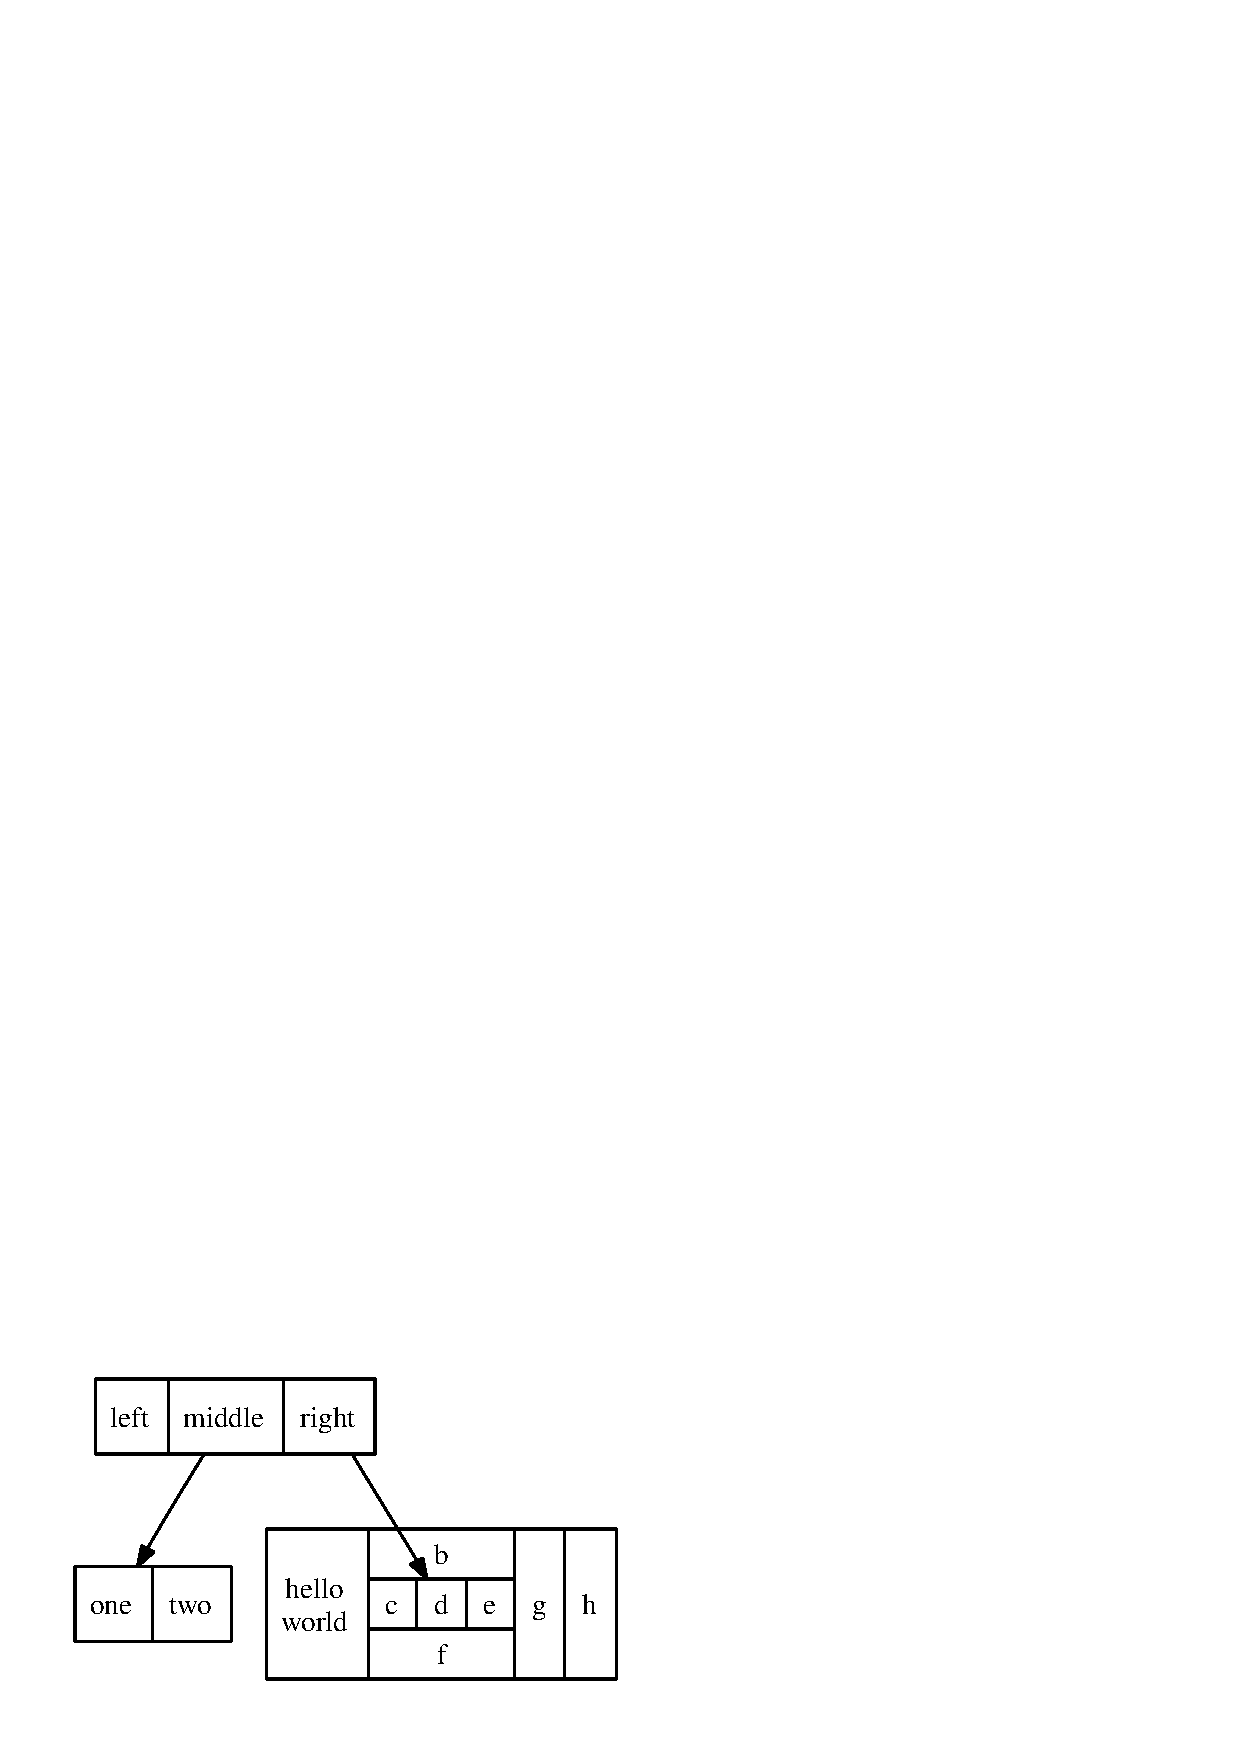
\includegraphics{structs}
	}
    \caption{Drawing of records (revisited)}
    \label{fig:structdrawing}
\end{figure}
The example of Figures~\ref{fig:hashtable} and \ref{fig:hashtabledrawing}
uses left-to-right drawing in a layout of a hash table.
\begin{figure}[p]\footnotesize
\begin{verbatim}
 1:  digraph G {
 2:    nodesep=.05;
 3:    rankdir=LR;
 4:    node [shape=record,width=.1,height=.1];
 5:  
 6:    node0 [label = "<f0> |<f1> |<f2> |<f3> |<f4> |<f5> |<f6> | ",height=2.5];
 7:    node [width = 1.5];
 8:    node1 [label = "{<n> n14 | 719 |<p> }"];
 9:    node2 [label = "{<n> a1  | 805 |<p> }"];
10:    node3 [label = "{<n> i9  | 718 |<p> }"];
11:    node4 [label = "{<n> e5  | 989 |<p> }"];
12:    node5 [label = "{<n> t20 | 959 |<p> }"] ;
13:    node6 [label = "{<n> o15 | 794 |<p> }"] ;
14:    node7 [label = "{<n> s19 | 659 |<p> }"] ;
15:  
16:    node0:f0 -> node1:n;
17:    node0:f1 -> node2:n;
18:    node0:f2 -> node3:n;
19:    node0:f5 -> node4:n;
20:    node0:f6 -> node5:n;
21:    node2:p -> node6:n;
22:    node4:p -> node7:n;
23:  }
\end{verbatim}\vspace*{-.25in}
\caption{Hash table graph file}
\label{fig:hashtable}
\end{figure}

\begin{figure}[p]
	\centerline {
		\includegraphics[height=2.5in]{hashtable}
	}
    \caption{Drawing of hash table}
    \label{fig:hashtabledrawing}
\end{figure}

\subsection{Clusters}

A cluster is a subgraph placed in its own distinct rectangle of the layout.
A subgraph is recognized as a cluster when its name has the prefix
\verb"cluster". (If the top-level graph has {\tt clusterrank=none},
this special processing is turned off).
Labels, font characteristics and the {\tt labelloc} attribute can 
be set as they would be for the top-level graph, though
cluster labels appear above the graph by default. 
For clusters, the label is left-justified by default;
if {\tt labeljust="r"}, the label is right-justified.
The {\tt color} attribute specifies the color of the enclosing rectangle.
In addition, clusters may have {\tt style="filled"}, in which case
the rectangle is filled with the color specified by {\tt fillcolor}
before the cluster is drawn. (If  {\tt fillcolor} is not specified,
the cluster's {\tt color} attribute is used.)

Clusters are drawn by a recursive technique that computes a
rank assignment and internal ordering of nodes within clusters.
Figure~\ref{fig:clust1} through \ref{fig:callgraph} are cluster layouts
and the corresponding graph files.

\begin{figure}[p]
\begin{minipage}[t]{2.5in}
\footnotesize
\begin{verbatim}
digraph G {
    subgraph cluster0 {
        node [style=filled,color=white];
        style=filled;
        color=lightgrey;
        a0 -> a1 -> a2 -> a3;
        label = "process #1";
    }

    subgraph cluster1 {
        node [style=filled];
        b0 -> b1 -> b2 -> b3;
        label = "process #2";
        color=blue
    }
    start -> a0;
    start -> b0;
    a1 -> b3;
    b2 -> a3;
    a3 -> a0;
    a3 -> end;
    b3 -> end;

    start [shape=Mdiamond];
    end [shape=Msquare];
}
\end{verbatim}
\end{minipage} \hspace{0.05in} \
\parbox[t]{2.0in}{
    \ \\
	\centerline {
		\includegraphics[width=1.9in]{clust1}
	}
}
    \caption{Process diagram with clusters}
    \label{fig:clust1}
\end{figure}
\clearpage

\begin{figure}[p]
\footnotesize
\begin{verbatim}
1:digraph G {
2:  size="8,6"; ratio=fill; node[fontsize=24];
3:
4:  ciafan->computefan; fan->increment; computefan->fan; stringdup->fatal;
5:  main->exit; main->interp_err; main->ciafan; main->fatal; main->malloc;
6:  main->strcpy; main->getopt; main->init_index; main->strlen; fan->fatal;
7:  fan->ref; fan->interp_err; ciafan->def; fan->free; computefan->stdprintf;
8:  computefan->get_sym_fields; fan->exit; fan->malloc; increment->strcmp;
9:  computefan->malloc; fan->stdsprintf; fan->strlen; computefan->strcmp;
10:  computefan->realloc; computefan->strlen; debug->sfprintf; debug->strcat;
11:  stringdup->malloc; fatal->sfprintf; stringdup->strcpy; stringdup->strlen;
12:  fatal->exit;
13:
14:  subgraph "cluster_error.h" { label="error.h"; interp_err; }
15:
16:  subgraph "cluster_sfio.h" { label="sfio.h"; sfprintf; }
17:
18:  subgraph "cluster_ciafan.c" { label="ciafan.c"; ciafan; computefan;
19:      increment; }
20:
21:  subgraph "cluster_util.c" { label="util.c"; stringdup; fatal; debug; }
22:
23:  subgraph "cluster_query.h" { label="query.h"; ref; def; }
24:
25:  subgraph "cluster_field.h" { get_sym_fields; }
26:
27:  subgraph "cluster_stdio.h" { label="stdio.h"; stdprintf; stdsprintf; }
28:
29:  subgraph "cluster_<libc.a>" { getopt; }
30:
31:  subgraph "cluster_stdlib.h" { label="stdlib.h"; exit; malloc; free; realloc; }
32:
33:  subgraph "cluster_main.c" { main; }
34:
35:  subgraph "cluster_index.h" { init_index; }
36:
37:  subgraph "cluster_string.h" { label="string.h"; strcpy; strlen; strcmp; strcat; }
38:}
\end{verbatim}
\caption{Call graph file}
\label{fig:clust2}
\end{figure}

\begin{figure}[p]
	\centerline {
		\includegraphics[width=6.5in]{clust2}
	}
    \caption{Call graph with labeled clusters}
	\label{fig:callgraph}
\end{figure}

If the top-level graph has the {\tt compound} attribute set to true,
\dot\ will allow edges connecting nodes and clusters. This is accomplished
by an edge defining an {\tt lhead} or {\tt ltail} attribute. The
value of these attributes must be the name of a cluster containing the
head or tail node, respectively. In this case, the edge is clipped at
the cluster boundary. All other edge attributes, such as {\tt arrowhead}
or {\tt dir}, are applied to the truncated edge. For example,
Figure~\ref{fig:compound} shows a graph using the {\tt compound} attribute
and the resulting diagram.

\begin{figure}[p]
\begin{minipage}[t]{2.25in}
\begin{verbatim}
digraph G {
    compound=true;
    subgraph cluster0 {
      a -> b;
      a -> c;
      b -> d;
      c -> d;
    }
    subgraph cluster1 {
      e -> g;
      e -> f;
    }
    b -> f [lhead=cluster1];
    d -> e;
    c -> g [ltail=cluster0,
             lhead=cluster1];
    c -> e [ltail=cluster0];
    d -> h;
}
\end{verbatim}
\end{minipage} \hspace{0.5in} \
\parbox[t]{2.0in}{
    \ \\
	\centerline {
		\includegraphics[width=2in]{compound}
	}
}
    \caption{Graph with edges on clusters}
    \label{fig:compound}
\end{figure}

\subsection{Concentrators}
Setting \verb"concentrate=true" on the top-level graph enables 
an edge merging technique to reduce clutter in dense layouts.
Edges are merged when they run parallel, have a common endpoint
and have length greater than 1.
A beneficial side-effect in fixed-sized layouts is that removal
of these edges often permits larger, more readable labels.
While concentrators in \dot\ look somewhat like Newbery's
\cite{newbery:concentrators}, they are found by searching
the edges in the layout, not by detecting complete bipartite graphs in
the underlying graph.  Thus the \dot\ approach runs much faster
but doesn't collapse as many edges as Newbery's algorithm.

\section{Command Line Options}

By default, \dot\ operates in filter mode,
reading a graph from {\tt stdin}, and
writing the graph on {\tt stdout} in the \DOT\ format with 
layout attributes appended.
\dot\ supports a variety of command-line options:

{\tt-T{\it format}} sets the format of the output. Allowed values
for {\it format} are:

\begin{description}
\item[{\tt bmp}] Windows bitmap format.
\item[{\tt canon}]
Prettyprint input; no layout is done.
\item[{\tt dot}] 
Attributed \DOT. Prints input with layout information attached as
attributes, cf. Appendix~\ref{sect:output}.
\item[{\tt fig}] FIG output.
\item[{\tt gd}] GD format. This is the internal format used by the GD Graphics
Library. An alternate format is {\tt gd2}.
\item[{\tt gif}] GIF output.
\item[{\tt imap}] Produces map files for server-side image 
maps. This can be combined with a graphical form of the output, e.g., using
{\tt -Tgif} or {\tt -Tjpg}, in web pages to attach links to nodes and edges. 
\item[{\tt cmapx}] Produces HTML map files for client-side image maps.
\item[{\tt pdf}] Adobe PDF via the Cairo library. We have seen problems when embedding into other documents. Instead, use -Tps2 as described below.
\item[{\tt plain}] Simple, line-based ASCII format. Appendix~\ref{app:plain}
describes this output. An alternate format is {\tt plain-ext}, which 
provides port names on the head and tail nodes of edges.
\item[{\tt png}] PNG (Portable Network Graphics) output.
\item[{\tt ps}] PostScript (EPSF) output.
\item[{\tt ps2}] PostScript (EPSF) output with PDF annotations. This output should be distilled into PDF, such as for pdflatex, before being included in 
a document. (Use ps2pdf; epstopdf doesn't handle \verb"%%BoundingBox: (atend)".)
\item[{\tt svg}] SVG output. The alternate form {\tt svgz} produces
compressed SVG.
\item[{\tt vrml}] VRML output.
\item[{\tt wbmp}] Wireless BitMap (WBMP) format.
\end{description}

{\tt-G{\it name}={\it value}} sets a graph attribute default value.
Often it is convenient to set size, pagination, and related
values on the command line rather than in the graph file.
The analogous flags \verb"-N" or \verb"-E" 
set default node or edge attributes.
Note that file contents override command line arguments.

{\tt-l{\it libfile}} specifies a device-dependent graphics library
file. Multiple libraries may be given. These names are passed to the code
generator at the beginning of output. 

{\tt-o{\it outfile}} writes output into file {\it outfile}.

\verb"-v" requests verbose output.  In processing large layouts,
the verbose messages may give some estimate of \dot's progress.

\verb"-V" prints the version number and exits.

\section{Miscellaneous}

In the top-level graph heading, a graph may be declared a
{\tt strict digraph} or a {\tt strict graph}. This forbids the creation 
of multi-edges, i.e., there can be at most one edge with a given tail
node and head node in the directed case. For undirected graphs, 
there can be at most one
edge connected to the same two nodes. Subsequent edge statements using
the same two nodes will identify the edge with the previously defined one
and apply any attributes given in the edge statement.

Nodes, edges and graphs may have a {\tt URL} attribute. In certain
output formats ({\tt ps2}, {\tt imap}, {\tt cmapx}, or {\tt svg}), 
this information is integrated in the output 
so that nodes, edges and clusters become active links
when displayed with the appropriate tools. Typically, URLs attached to
top-level graphs serve as base URLs, supporting relative URLs on
components. When the output format is {\tt imap}, or {\tt cmapx},
a similar processing
takes place with the {\tt headURL} and {\tt tailURL} attributes.

For certain formats ({\tt ps}, {\tt fig} 
or {\tt svg}), {\tt comment} attributes can be used to
embed human-readable notations in the output.

\section{Conclusions}

\dot\ produces pleasing hierarchical drawings and can be
applied in many settings.

Since the basic algorithms of \dot\ work well, we have a good basis for
further research into problems such as methods for drawing large graphs
and on-line (animated) graph drawing.

\section{Acknowledgments}
We thank Phong Vo for his advice
about graph drawing algorithms and programming.
The graph library uses Phong's splay tree dictionary library.
Also, the users of \dag, the predecessor of \dot, 
gave us many good suggestions.
Guy Jacobson and Randy Hackbarth reviewed earlier
drafts of this manual, and Emden contributed substantially to the
current revision.  John Ellson wrote the generalized polygon
shape and spent considerable effort to make it robust and efficient.
He also wrote the GIF and ISMAP generators and other tools
to bring \graphviz\ to the web.

\clearpage
\bibliography{graphdraw} 

\appendix
\clearpage
\section{Principal Node Attributes}
\label{sec:node_attr}
%\begin{table}[p]
\begin{tabular}[t]{|l|l|p{3.0in}|} \hline
Name & Default & Values \\ \hline
%{\tt bottomlabel} & & auxiliary label for nodes of {\tt shape} M* \\
{\tt color} & {\tt black} & node shape color \\
{\tt colorscheme} & X11 & scheme for interpreting color names \\
{\tt comment} & & any string (format-dependent) \\
{\tt distortion} & {\tt 0.0} & node distortion for {\tt shape=polygon} \\
{\tt fillcolor} & {\tt lightgrey/black} & node fill color \\
{\tt fixedsize} & false & label text has no affect on node size \\
{\tt fontcolor} & {\tt black} & type face color \\
{\tt fontname} & {\tt Times-Roman} & font family \\
{\tt fontsize} & {\tt 14} & point size of label \\
{\tt group} &  & name of node's horizontal alignment group \\
{\tt height} & {\tt .5} & minimum height in inches \\
{\tt id} & & any string (user-defined output object tags) \\
{\tt image} & & image file name \\
{\tt imagescale} & false & true, width, height, both \\
{\tt label} & node name & any string \\
{\tt labelloc} & c & node label vertical alignment \\
{\tt layer} & overlay range & {\tt all}, {\it id} or {\it id:id}, or a comma-separated
list of the former \\
{\tt margin} & 0.11,0.55 & space around label \\
{\tt nojustify} & false & if true, justify to label, not node \\
{\tt orientation} & {\tt 0.0} & node rotation angle \\
{\tt penwidth} & 1.0 & width of pen for drawing boundaries, in points \\
{\tt peripheries} & {\tt shape-dependent} & number of node boundaries \\
{\tt regular} & false & force polygon to be regular \\
{\tt samplepoints} & 8 or 20 & number vertices to convert circle or ellipse \\
{\tt shape} & {\tt ellipse} & node shape; see Section~\ref{sect:shape} and
Appendix~\ref{app:shapes}\\
% {\tt shapefile} & & (deprecated, shape file)\\
{\tt sides} & {\tt 4} & number of sides for {\tt shape=polygon} \\
{\tt skew} & {\tt 0.0} & skewing of node for {\tt shape=polygon} \\
{\tt style} & & graphics options, e.g. {\tt bold, dotted, filled};
cf. Section~\ref{sect:style} \\ 
{\tt target} & & if URL is set, determines browser window for URL \\
{\tt tooltip} & label & tooltip annotation \\
%{\tt toplabel} & & auxiliary label for nodes of {\tt shape} M* \\
{\tt URL} & & URL associated with node (format-dependent) \\
{\tt width} & {\tt .75} & minimum width in inches \\
\hline
\end{tabular}
%\caption{Node attributes}
%\label{tab:nattr}
%\end{table}

%\clearpage
\section{Principal Edge Attributes}
\label{sec:edge_attr}
%\begin{table}[p]
{\footnotesize
\begin{tabular}[t]{|l|l|p{3.5in}|} \hline
Name & Default & Values \\ \hline
{\tt arrowhead} & normal & style of arrowhead at head end \\
{\tt arrowsize} & {\tt 1.0} & scaling factor for arrowheads \\
{\tt arrowtail} & normal & style of arrowhead at tail end \\
{\tt color} & {\tt black} & edge stroke color \\
{\tt colorscheme} & X11 & scheme for interpreting color names \\
{\tt comment} & & any string (format-dependent) \\
{\tt constraint} & true & use edge to affect node ranking \\
{\tt decorate} & & if set, draws a line connecting labels with their edges \\
{\tt dir} & {\tt forward} & {\tt forward}, {\tt back}, {\tt both}, or {\tt none} \\ 
{\tt edgeURL} & & URL attached to non-label part of edge \\
{\tt edgehref} & & synonym for edgeURL \\
{\tt edgetarget} & & if URL is set, determines browser window for URL \\
{\tt edgetooltip} & label & tooltip annotation for non-label part of edge \\
{\tt fontcolor} & {\tt black} & type face color \\
{\tt fontname} & {\tt Times-Roman} & font family \\
{\tt fontsize} & {\tt 14} & point size of label \\
{\tt headclip} & true & if false, edge is not clipped to head node boundary \\
{\tt headhref} & & synonym for headURL \\
{\tt headlabel} & & label placed near head of edge \\
{\tt headport} & & {\tt n,ne,e,se,s,sw,w,nw}\\
{\tt headtarget} & & if headURL is set, determines browser window for URL \\
{\tt headtooltip} & label & tooltip annotation near head of edge \\
{\tt headURL} & & URL attached to head label \\
{\tt href} & & alias for URL \\
{\tt id} & & any string (user-defined output object tags) \\
{\tt label} & & edge label \\
{\tt labelangle} & {\tt -25.0} & angle in degrees which head or tail label
is rotated off edge \\
{\tt labeldistance} & {\tt 1.0} & scaling factor for distance of head or tail label from node \\
{\tt labelfloat} & false & lessen constraints on edge label placement \\
{\tt labelfontcolor} & {\tt black} & type face color for head and tail labels\\
{\tt labelfontname} & {\tt Times-Roman} & font family for head and tail labels\\
{\tt labelfontsize} & {\tt 14} & point size for head and tail labels \\
{\tt labelhref} & & synonym for labelURL \\
{\tt labelURL} & & URL for label, overrides edge URL \\
{\tt labeltarget} & & if URL or labelURL is set, determines browser window for URL \\
{\tt labeltooltip} & label & tooltip annotation near label \\
{\tt layer} & overlay range & {\tt all}, {\it id} or {\it id:id}, or a comma-separated
list of the former\\
{\tt lhead} & & name of cluster to use as head of edge \\
{\tt ltail} & & name of cluster to use as tail of edge \\
{\tt minlen} & {\tt 1} & minimum rank distance between head and tail \\
{\tt penwidth} & 1.0 & width of pen for drawing edge stroke, in points \\
{\tt samehead} & & tag for head node; edge heads with the same tag are merged onto
the same port \\
{\tt sametail} & & tag for tail node; edge tails with the same tag are merged onto
the same port \\
{\tt style} & & graphics options, e.g. {\tt bold, dotted, filled}; cf.
Section~\ref{sect:style} \\ 
{\tt tailclip} & true & if false, edge is not clipped to tail node boundary \\
{\tt tailhref} & & synonym for tailURL \\
{\tt taillabel} & & label placed near tail of edge \\
{\tt tailport} & & {\tt n,ne,e,se,s,sw,w,nw}\\
{\tt tailtarget} & & if tailURL is set, determines browser window for URL \\
{\tt tailtooltip} & label & tooltip annotation near tail of edge \\
{\tt tailURL} & & URL attached to tail label \\
{\tt target} & & if URL is set, determines browser window for URL \\
{\tt tooltip} & label & tooltip annotation \\
{\tt weight} & {\tt 1} & integer cost of stretching an edge \\
\hline
\end{tabular}
%\caption{Edge attributes}
%\label{tab:eattr}
%\end{table}
}

%\clearpage
\section{Principal Graph Attributes}
\label{sec:graph_attr}

%\begin{table}[p]
{\footnotesize
\begin{tabular}[t]{|l|l|p{3.5in}|} \hline
Name & Default & Values \\ \hline
{\tt aspect} &  & controls aspect ratio adjustment \\
{\tt bgcolor} &  & background color for drawing, plus initial fill color \\
{\tt center} & false & center drawing on {\tt page} \\ 
{\tt clusterrank} & {\tt local} & may be {\tt global} or {\tt none} \\
{\tt color} & {\tt black} & for clusters, outline color, and fill color
if {\tt fillcolor} not defined \\
{\tt colorscheme} & X11 & scheme for interpreting color names \\
{\tt comment} & & any string (format-dependent) \\
{\tt compound} & false & allow edges between clusters \\
{\tt concentrate} & false & enables edge concentrators  \\ 
{\tt dpi} & 96 & dots per inch for image output \\
{\tt fillcolor} & {\tt black} & cluster fill color \\
{\tt fontcolor} & {\tt black} & type face color \\ 
{\tt fontname} & {\tt Times-Roman} & font family \\
{\tt fontnames} & & {\tt svg}, {\tt ps}, {\tt gd} (SVG only) \\
{\tt fontpath} &  & list of directories to search for fonts \\
{\tt fontsize} & {\tt 14} & point size of label \\
{\tt id} & & any string (user-defined output object tags) \\
{\tt label} & & any string \\
{\tt labeljust} & centered & "l" and "r" for left- and right-justified 
cluster labels, respectively \\
{\tt labelloc} & top & "t" and "b" for top- and bottom-justified cluster 
labels, respectively \\
{\tt landscape} & & if true, means orientation=landscape \\
{\tt layers} & & {\it id:id:id...} \\
{\tt layersep} & : & specifies separator character to split {\tt layers} \\
{\tt margin} & {\tt .5} & margin included in {\tt page}, inches \\
{\tt mindist} & {\tt 1.0} & minimum separation between all nodes (not dot)\\
{\tt nodesep} & {\tt .25} & separation between nodes, in inches. \\
{\tt nojustify} & false & if true, justify to label, not graph \\
{\tt ordering} & & if {\tt out} out edge order is preserved \\
{\tt orientation} & {\tt portrait} & if {\tt rotate} is not used and the value
is {\tt landscape}, use landscape orientation \\
{\tt outputorder} & breadthfirst & or nodesfirst, edgesfirst \\
{\tt page} & & unit of pagination, {\it e.g.} {\tt "8.5,11"} \\
{\tt pagedir} & {\tt BL} & traversal order of pages \\
{\tt pencolor} & black & color for drawing cluster boundaries \\
{\tt penwidth} & 1.0 & width of pen for drawing boundaries, in points \\
{\tt peripheries} & 1 & number of cluster boundaries \\
{\tt rank} & & {\tt same}, {\tt min}, {\tt max}, {\tt source} or {\tt sink} \\
{\tt rankdir} & {\tt TB} & {\tt LR} (left to right) or {\tt TB} (top to bottom) \\
{\tt ranksep} & {\tt .75} & separation between ranks, in inches. \\
{\tt ratio} & & approximate aspect ratio desired, {\tt fill} or {\tt auto} \\
minimization \\
{\tt rotate} & & If 90, set orientation to landscape \\
{\tt samplepoints} & {\tt 8} & number of points used to represent ellipses
and circles on output (cf.  Appendix~\ref{sect:output} \\
{\tt searchsize} & {\tt 30} & maximum edges with negative cut values to
check when looking for a minimum one during network simplex \\
{\tt size} & & maximum drawing size, in inches \\
{\tt splines} & & draw edges as splines, polylines, lines \\
{\tt style} & & graphics options, e.g. {\tt filled} for clusters \\
{\tt stylesheet} & & pathname or URL to XML style sheet for SVG \\
{\tt target} & & if URL is set, determines browser window for URL \\
{\tt tooltip} & label & tooltip annotation for cluster \\
{\tt truecolor} &  & if set, force 24 bit or indexed color in image output \\
{\tt viewport} &  & clipping window on output \\
{\tt URL} & & URL associated with graph (format-dependent) \\
\hline
\end{tabular}
%\caption{Graph attributes}
%\label{tab:gattr}
%\end{table}
}

\clearpage
\section{Graph File Grammar}
\label{grammar}

\newcommand{\lopt}{[}
\newcommand{\ropt}{]}
\newcommand{\lgrp}{(}
\newcommand{\rgrp}{)}
\newcommand{\strict}{{\bf strict}}
\newcommand{\graph}{{\bf graph}}
\newcommand{\digraph}{{\bf digraph}}
\newcommand{\node}{{\bf node}}
\newcommand{\edge}{{\bf edge}}
\newcommand{\subgraph}{{\bf subgraph}}

The following is an abstract grammar for the \DOT\ language.
Terminals are shown in bold font and nonterminals in italics.
Literal characters are given in single quotes.
Parentheses \lgrp\ and \rgrp\ indicate grouping when needed.
Square brackets \lopt\ and \ropt\ enclose optional items.
Vertical bars $|$ separate alternatives.

\begin{tabular}{lll}

{\it graph}  & $\rightarrow$ & \lopt \strict \ropt\ \lgrp\digraph\ $|$ \graph\rgrp\ {\it id} '\{' {\it stmt-list} '\}' \\

{\it stmt-list} & $\rightarrow$ & \lopt {\it stmt} \lopt';'\ropt\  \lopt {\it stmt-list}\ \ropt\ \ropt \\

{\it stmt} & $\rightarrow$ & {\it attr-stmt} $|$ {\it node-stmt} $|$ {\it edge-stmt} $|$ {\it subgraph} $|$ {\it id} '=' {\it id} \\

{\it attr-stmt} & $\rightarrow$ & \lgrp\graph\ $|$ \node\ $|$ \edge\rgrp\ {\it attr-list} \\

{\it attr-list} & $\rightarrow$ & '[' \lopt {\it a-list} \ropt\ ']' \lopt {\it attr-list}\ropt \\

{\it a-list} & $\rightarrow$ & {\it id} '=' {\it id} \lopt','\ropt\ \lopt {\it a-list}\ropt \\

{\it node-stmt} & $\rightarrow$ & {\it node-id} \lopt{\it attr-list}\ropt \\

{\it node-id}  & $\rightarrow$ & {\it id} \lopt  {\it port}\ropt \\
{\it port}  & $\rightarrow$ & {\it port-location} \lopt  {\it port-angle}\ropt\
 $|$ {\it port-angle} \lopt  {\it port-location}\ropt \\

{\it port-location}  & $\rightarrow$ & ':' {\it id} $|$ ':' '(' {\it id} ',' {\it id} ')' \\
{\it port-angle}  & $\rightarrow$ & '@' {\it id} \\

{\it edge-stmt} & $\rightarrow$ & \lgrp{\it node-id} $|$ {\it subgraph}\rgrp\ {\it edgeRHS} \lopt {\it attr-list}\ropt \\

{\it edgeRHS} & $\rightarrow$ & {\it edgeop} \lgrp{\it node-id} $|$ {\it subgraph}\rgrp\ \lopt {\it edgeRHS}\ropt \\

{\it subgraph} & $\rightarrow$ & \lopt \subgraph\ {\it id}\ropt\ '\{' {\it stmt-list} '\}' $|$ \subgraph\ {\it id} \\

\end{tabular}

An {\it id} is any alphanumeric string not beginning with a digit,
but possibly including underscores; or a number; or any quoted
string possibly containing escaped quotes.

An {\it edgeop} is \verb"->" in directed graphs and \verb"--" in
undirected graphs.

The language supports C++-style comments: \verb"/* */" and \verb"//". 

Semicolons aid readability but are not required except in the rare case
that a named subgraph with no body immediate precedes an anonymous
subgraph, because under precedence rules this sequence is parsed as
a subgraph with a heading and a body.

Complex attribute values may contain characters, such as commas and
white space, which are used in parsing the \DOT\ language. To avoid getting
a parsing error, such values need to be enclosed in double quotes.

\clearpage
\section{Plain Output File Format ({\tt -Tplain})}
\label{app:plain}
{
\parindent0pt

The ``plain'' output format of \dot\ lists node and edge
information in a simple, line-oriented style which is easy
to parse by front-end components.
All coordinates and lengths are unscaled and in inches.

The first line is:

\hspace{.5in}\verb"graph" {\it scalefactor width height}

The {\it width} and {\it height} values give the width and the height
of the drawing; the lower-left corner of the drawing is at the origin.
The {\it scalefactor} indicates how much to scale all coordinates
in the final drawing.

The next group of lines lists the nodes in the format:

\hspace{.5in}\verb"node" {\it name x y xsize ysize label style shape color fillcolor }

The {\it name} is a unique identifier. If it contains whitespace or
punctuation, it is quoted. The {\it x} and {\it y} values give the coordinates
of the center of the node; the {\it width} and {\it height} give the 
width and the height. The remaining parameters provide the node's
{\tt label}, {\tt style}, {\tt shape}, {\tt color} and {\tt fillcolor} 
attributes, respectively. If the node does not have a {\tt style} attribute,
{\tt "solid"} is used. 

The next group of lines lists edges:

\hspace{.5in}\verb"edge" {\it tail head $n$ $x_1$ $y_1$ $x_2$ $y_2$
$\ldots$ $x_n$ $y_n$ {\rm [} label lx ly {\rm ]} style color }

$n$ is the number of coordinate pairs that follow as B-spline
control points.  If the edge is labeled, then the label text and
coordinates are listed next. The edge description is completed by 
the edge's {\tt style} and {\tt color}. As with nodes, if a {\tt style} is not
defined, {\tt "solid"} is used. 

The last line is always:

\hspace{.5in}\verb"stop"
}

\clearpage
\section{Attributed \DOT\ Format ({\tt -Tdot})}
\label{sect:output}

This is the default output format. It reproduces the input, 
along with layout information for the graph. Coordinate values
increase up and to the right. Positions are represented by two
integers separated by a comma, representing the $X$ and $Y$ coordinates
of the location specified in points (1/72 of an inch). A position
refers to the center of its associated object.
Lengths are given in inches.

A {\tt bb} attribute is attached to the graph, 
specifying the bounding box of the drawing. If the graph has a label, 
its position is specified by the {\tt lp} attribute. 

Each node gets {\tt pos}, {\tt width} and {\tt height} attributes. 
If the node is a record, the record rectangles are given in the {\tt rects}
attribute. If the node is polygonal and the {\tt vertices} 
attribute is defined in the input graph, this attribute contains the 
vertices of the node. The number of points produced for circles and ellipses
is governed by the {\tt samplepoints} attribute.

Every edge is assigned a {\tt pos} attribute, which consists of
a list of $3n + 1$ locations. These are B-spline control points:
points $p_0, p_1, p_2, p_3$ are the first Bezier spline,
$p_3, p_4, p_5, p_6$ are the second, etc.
Currently, edge points are listed top-to-bottom (or left-to-right)
regardless of the orientation of the edge. This may change.

In the {\tt pos} attribute, the list of control points might
be preceded by a start point $p_s$ and/or an end point $p_e$. These have the
usual position representation with a {\tt "s,"} or {\tt "e,"}
prefix, respectively. A start point is present if there is an 
arrow at $p_0$.
In this case, the arrow is from $p_0$ to $p_s$, where
$p_s$ is actually on the node's boundary. The length and direction
of the arrowhead
is given by the vector $(p_s - p_0)$.
If there is no arrow, $p_0$ is on the node's boundary.
Similarly, the point $p_e$ designates an arrow at the other end of the
edge, connecting to the last spline point.

If the edge has a label, the label position is given in {\tt lp}. 

\clearpage
\section{Layers}
{\dot} has a feature for drawing parts of a single diagram on
a sequence of overlapping ``layers.'' Typically the layers are
overhead transparencies.  To activate this feature, one must
set the top-level graph's {\tt layers} attribute to a list of identifiers.
A node or edge can then be assigned to list of layers
using its {\tt layer} attribute.
A list of layers is specified as a comma-separated list of ranges, and
a range is either a single layer or has the form {\em id}:{\em id'}, the latter
denoting all layers from {\em id} through {\em id'}.
{\tt all} is a reserved name for all layers (and can be
used at either end of a range, e.g {\tt design:all} or {\tt all:code}).
For example:
\begin{verbatim}
    layers = "spec:design:code:debug:ship";
    node90 [layer = "code"];
    node91 [layer = "design:debug"]; 
    node92 [layer = "all:code"];
    node93 [layer = "spec:code,ship"];
    node90 -> node91 [layer = "all"];
\end{verbatim}
In this graph, {\tt node91} is in layers {\tt design}, {\tt code}
and {\tt debug}, while {\tt node92} is in layers {\tt spec},
{\tt design} and {\tt code}. {\tt node93} is in layers
layers {\tt spec}, {\tt design}, {\tt code} and {\tt ship}.

In a layered graph, if a node or edge has no layer assignment,
but incident edges or nodes do, then its layer specification
is inferred from these.  To change the default so that nodes
and edges with no layer appear on all layers, insert near
the beginning of the graph file:

\begin{verbatim}
    node [layer=all];
    edge [layer=all];
\end{verbatim}

When PostScript output is selected, the color sequence for layers
is set in the array {\tt layercolorseq}.  This array is indexed
starting from 1, and every element must be a 3-element array which can
interpreted as a color coordinate.  The adventurous may
learn further from reading {\dot}'s PostScript output.

\clearpage  % why does this create a blank page here?
\section{Node Shapes}
\label{app:shapes}
These are the principal node shapes. A more complete description of
node shapes can be found at the web site
\begin{center}
{\tt www.graphviz.org/doc/info/shapes.html}
\end{center}
%\vspace{0.15in}
\begin{center}
\begin{tabular}{cccc}\footnotesize

\includegraphics{box} & 
\includegraphics{polygon} & 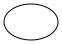
\includegraphics{ellipse} & 
\includegraphics{circle} \\
box & polygon & ellipse & circle \\

\includegraphics{point} & 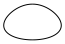
\includegraphics{egg} & 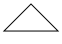
\includegraphics{triangle} & 
\includegraphics{plaintext} \\
point & egg & triangle & plaintext \\
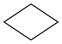
\includegraphics{diamond} & 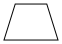
\includegraphics{trapezium} & 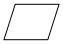
\includegraphics{parallelogram} & 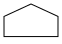
\includegraphics{house} \\
diamond & trapezium & parallelogram & house \\
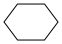
\includegraphics{hexagon} & 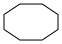
\includegraphics{octagon} & 
\includegraphics{doublecircle} & 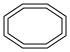
\includegraphics{doubleoctagon} \\ 
hexagon & octagon & doublecircle & doubleoctagon  \\
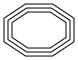
\includegraphics{tripleoctagon} & 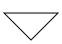
\includegraphics{invtriangle} & 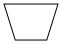
\includegraphics{invtrapezium} & 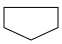
\includegraphics{invhouse} \\
tripleoctagon & invtriangle & invtrapezium & invhouse \\
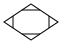
\includegraphics{Mdiamond} & 
\includegraphics{Msquare} & 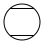
\includegraphics{Mcircle} & 
\includegraphics{none} \\
Mdiamond & Msquare & Mcircle & none \\
\includegraphics[scale=0.5]{record} &  \includegraphics[scale=0.5]{Mrecord} & & \\
record  & Mrecord & & \\
\end{tabular}
\end{center}

\clearpage
\section{Arrowhead Types}
\label{app:arrows}
These are some of the main arrowhead types. A more complete description of
these shapes can be found at the web site
\begin{center}
{\tt www.graphviz.org/doc/info/arrows.html}
\end{center}
\begin{center}
\begin{tabular}{ccc}
\includegraphics{normal} & 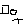
\includegraphics{dot} & \includegraphics{inv} \\
normal & dot & inv \\
\includegraphics{crow} & \includegraphics{tee} & \includegraphics{vee} \\
crow & tee & vee \\
\includegraphics{diamondarrow} & \includegraphics{no_arrow} & \includegraphics{boxarrow} \\
diamond & none & box \\
\includegraphics{curve} & \includegraphics{icurve} & \\
curve & icurve & \\
\end{tabular}
\end{center}
Arrowhead descriptions support a simple grammar to allow more complex, derived shapes,
such as the examples below.
\begin{center}
\begin{tabular}{ccc}
\includegraphics{odot} & \includegraphics{invdot} & \includegraphics{invodot} \\
odot & invdot & invodot \\
\end{tabular}
\end{center}
The web page cited above describes this grammar in detail.

\clearpage
\section{Color Names}
\label{app:colors}
Here are some basic color names. More information about colors
can be found at
\begin{center}
{\tt www.graphviz.org/doc/info/colors.html} \\
{\tt www.graphviz.org/doc/info/attrs.html\#k:color}
\end{center}
{\footnotesize
\begin{tabular*}{\textwidth}{@{\extracolsep{\fill}}llll}
{\bf Whites} & {\bf  Reds} & {\bf  Yellows} & turquoise[1-4] \cr
antiquewhite[1-4] & coral[1-4] & darkgoldenrod[1-4] \cr
azure[1-4] & crimson & gold[1-4] & {\bf  Blues} \cr
bisque[1-4] & darksalmon & goldenrod[1-4] & aliceblue \cr
blanchedalmond & deeppink[1-4] & greenyellow & blue[1-4] \cr
cornsilk[1-4] & firebrick[1-4] & lightgoldenrod[1-4] & blueviolet \cr
floralwhite & hotpink[1-4] & lightgoldenrodyellow & cadetblue[1-4] \cr
gainsboro & indianred[1-4] & lightyellow[1-4] & cornflowerblue \cr
ghostwhite & lightpink[1-4] & palegoldenrod & darkslateblue \cr
honeydew[1-4] & lightsalmon[1-4] & yellow[1-4] & deepskyblue[1-4] \cr
ivory[1-4] & maroon[1-4] & yellowgreen & dodgerblue[1-4] \cr
lavender & mediumvioletred & & indigo \cr
lavenderblush[1-4] & orangered[1-4] & {\bf  Greens} & lightblue[1-4] \cr
lemonchiffon[1-4] & palevioletred[1-4] & chartreuse[1-4] & lightskyblue[1-4] \cr
linen & pink[1-4] & darkgreen & lightslateblue[1-4] \cr
mintcream & red[1-4] & darkolivegreen[1-4] & mediumblue \cr
mistyrose[1-4] & salmon[1-4] & darkseagreen[1-4] & mediumslateblue \cr
moccasin & tomato[1-4] & forestgreen & midnightblue \cr
navajowhite[1-4] & violetred[1-4] & green[1-4] & navy \cr
oldlace & & greenyellow & navyblue \cr
papayawhip & {\bf  Browns} & lawngreen & powderblue \cr
peachpuff[1-4] & beige & lightseagreen & royalblue[1-4] \cr
seashell[1-4] & brown[1-4] & limegreen & skyblue[1-4] \cr
snow[1-4] & burlywood[1-4] & mediumseagreen & slateblue[1-4] \cr
thistle[1-4] & chocolate[1-4] & mediumspringgreen & steelblue[1-4] \cr
wheat[1-4] & darkkhaki & mintcream \cr
white & khaki[1-4] & olivedrab[1-4] & {\bf  Magentas} \cr
whitesmoke & peru & palegreen[1-4] & blueviolet \cr
 & rosybrown[1-4] & seagreen[1-4] & darkorchid[1-4] \cr
{\bf  Greys} & saddlebrown & springgreen[1-4] & darkviolet \cr
darkslategray[1-4] & sandybrown & yellowgreen & magenta[1-4] \cr
dimgray & sienna[1-4] & & mediumorchid[1-4] \cr
gray & tan[1-4] & {\bf  Cyans} & mediumpurple[1-4] \cr
gray[0-100] & & aquamarine[1-4] & mediumvioletred \cr
lightgray & {\bf  Oranges} & cyan[1-4] & orchid[1-4] \cr
lightslategray & darkorange[1-4] & darkturquoise & palevioletred[1-4] \cr
slategray[1-4] & orange[1-4] & lightcyan[1-4] & plum[1-4] \cr
 & orangered[1-4] & mediumaquamarine & purple[1-4] \cr
{\bf  Blacks} & & mediumturquoise & violet \cr
black & & paleturquoise[1-4] & violetred[1-4] \cr
\end{tabular*}
}

%\tableofcontents
%\coversheet 
\end{document} 
% 
%END
